% -----------------------------------------------------------------------------
%
% Copyright (c) 2017 Sam Cox, Roberto Sommariva
%
% This file is part of the AtChem2 software package.
%
% This file is covered by the MIT license which can be found in the file
% LICENSE.md at the top level of the AtChem2 distribution.
%
% -----------------------------------------------------------------------------

\chapter{Model Execution} \label{ch:execution}

% -------------------------------------------------------------------- %
\section{Box-Model} \label{sec:box-model}

AtChem2 is a modelling tool to build and run atmospheric chemistry
box-models \citep{sommariva_2020}. The structure and organization of
AtChem2 are described in Sect.~\ref{sec:model-structure}. An AtChem2
box-model requires two sets of inputs, which are provided by the user:
the chemical mechanism file and the configuration files settings --
both are described in the following sections. Additionally, the model
can be constrained to observational data, as explained in
Sect.~\ref{sec:constraints}.

\subsection{Mechanism file} \label{subsec:mechanism-file}

AtChem2 is designed to use the \href{http://mcm.leeds.ac.uk/MCM/}{MCM}
as a chemical mechanism; other chemical mechanisms can be used, as
long as they are in the correct format.

The chemical mechanism must be provided as a text file in
\hyperref[subsec:facsimile-format]{FACSIMILE format}, with the
extension \texttt{.fac}). The mechanism file can be downloaded from
the MCM website using the \hyperref[subsec:mcm-extraction]{extraction
  tool} or it can be assembled manually. The user can modify the
\texttt{.fac} file with a text editor, if needed.

The \texttt{.fac} file is converted into a pre-compiled shared library
-- called \texttt{mechanism.so} -- and several mechanism files in
Fortran compatible format. These files are created during the
\hyperref[subsec:build-process]{build process} in the \sharedir\ (by
default, \texttt{model/configuration/}).

\subsection{Configuration files} \label{subsec:configuration-files}

The configuration of the box-model is set via a number of text files,
which can be modified by the user with a text editor. Detailed
information on the configuration files can be found in the
corresponding section:

\begin{itemize}
\item Model and solver parameters settings-- go to
  \hyperref[sec:model-parameters]{Model Parameters} and
  \hyperref[sec:solver-parameters]{Solver Parameters}.
\item Environment variables settings -- go to
  \hyperref[sec:environment-variables]{Environment Variables}.
\item Photolysis rates settings -- go to
  \hyperref[sec:photolysis-rates]{Photolysis Rates}.
\item Model initialization, input and output -- go to
  \hyperref[sec:config-files]{Config Files}.
\end{itemize}

% -------------------------------------------------------------------- %
\section{Constraints} \label{sec:constraints}

AtChem2 can be run in two modes:

\begin{itemize}
\item Unconstrained: all variables are calculated by the model from
  the initial conditions, which are set in the
  \hyperref[subsec:configuration-files]{configuration files}.
\item Constrained: one or more variables are constrained, meaning that
  the solver forces their value to a given value at each time
  step. The variables that are not constrained are calculated by the
  model.
\end{itemize}

The constraint data must be provided as one file for each constrained
variable, with the format described below. By default, the files with
the constraint data are located in \texttt{model/constraints/species/}
for the chemical species, \texttt{model/constraints/environment/} for
the environment variables, \texttt{model/constraints/photolysis/} for
the photolysis rates~\footnote{Although \texttt{JFAC} is an
  environment variable, the \texttt{JFAC} constraint file must be in
  the \texttt{constraints/photolysis/} directory.}. The default
directories can be changed, as explained Sect.~\ref{sec:build} (see
also Sect.~\ref{subsec:model-directory}).

\subsection{Constrained variables} \label{subsec:constrained-variables}

\subsubsection{Environment variables}

All environment variables, except \texttt{DILUTE} and \texttt{ROOF},
can be constrained. To do so, set the variable to \texttt{CONSTRAINED}
in \texttt{environmentVariables.config} and create a file with the
constraint data (Sect.~\ref{subsec:constraint-files}). The name of the
file must be the same as the name of the variable -- e.g.,
\texttt{TEMP} (without extension).

\subsubsection{Chemical species}

Any chemical species in the chemical mechanism can be constrained. To
do so, add the name of the species to
\texttt{speciesConstrained.config} and create a file with the
constraint data (Sect.~\ref{subsec:constraint-files}). The name of the
file must be the same as the name of the chemical species -- e.g.,
\texttt{O3} (without extension).

\subsubsection{Photolysis rates}

Any photolysis rate in the chemical mechanism can be constrained. The
photolysis rates are identified as \texttt{J<i>}, where \texttt{i} is
the ID number assigned by the MCM to each photolysis reaction
(Sect.~\ref{sec:photolysis-rates}). To constrain a photolysis rate add
its name to \texttt{photolysisConstrained.config} and create a file
with the constraint data (Sect.~\ref{subsec:constraint-files}). The
name of the file must be the same as the name of the photolysis rate
-- e.g., \texttt{J4} (without extension).

\subsection{Constraint files} \label{subsec:constraint-files}

The files with the constraint data are text files with two columns and
no header: the first column is the time in seconds from midnight of
the start date (in UTC, Sect.~\ref{sec:model-parameters}), the second
column is the value of the variable in the appropriate unit. For the
chemical species the unit is molecule cm$^{-3}$ and for the photolysis
rates the unit is s$^{-1}$; for the units of the environment
variables, see Sect.~\ref{sec:environment-variables}. For example:

\begin{verbatim}
-900   73.21
0      74.393
900    72.973
1800   72.63
2700   72.73
3600   69.326
4500   65.822
5400   63.83
6300   64.852
7200   64.739
\end{verbatim}

The time in the first column of a constraint file can be negative.
AtChem2 interprets negative times as ``seconds before midnight of the
start date''. Having data points with negative time can be useful to
allow correct interpolation of the variables at the beginning of the
model run. This is because the model constraints \emph{must cover} the
same amount of time, or preferably more, as the intended model runtime
to avoid interpolation errors -- see Sect.~\ref{subsec:interpolation}
for details.

For example: if the model starts at 41400 seconds (day 1 at 11:30) and
stops at 225900 seconds (day 3 at 14:45), then the first and the last
data points of a constraint file must have a time of 41400 seconds (or
lower) and 225900 seconds (or higher), respectively.

\subsection{Interpolation} \label{subsec:interpolation}

Constraints can be provided at different timescales. Typically, the
constraint data come from direct measurements and it is very common
for different instruments to sample with different frequencies. For
example, ozone (\cf{O3}) and nitrogen oxides (\cf{NO}, \cf{NO2}) can
be measured once every minute, but most hydrocarbons can be measured
only once every 30-60 minutes. The user can average the constraints so
that they are all with the same timescale, or can use the constraint
data with the original timescales. Both approaches have advantages and
disadvantages in terms of how much pre-processing work is required,
and in terms of model accuracy and integration speed: for more
information, see the discussion in \citet{sommariva_2020}. It is up to
the user to decide which approach is more suitable, based on the
objectives of the modelling work and on the available computing
resources.

Whether all the constraints have the same timescale or not, AtChem2
interpolates between data points using the interpolation method
selected in \texttt{model.parameters} (Sect.~\ref{sec:model-parameters}).
The default interpolation method is piecewise linear, but piecewise
constant interpolation is also available. The photolysis rates and the
environment variables are evaluated by the solver when needed -- each
is interpolated individually, only when constrained. This happens each
time the function \texttt{mechanism\_rates()} is called from
\texttt{FCVFUN()}, and is controlled by CVODE as it carries out the
integration. In a similar way, the interpolation routine for the
chemical species is called once for each of the constrained species in
\texttt{FCVFUN()}, plus once when setting the initial conditions of
each of the constrained species.

As mentioned in Sect.~\ref{subsec:constraint-files}, the model start
and stop times \emph{must be} within the time interval of all the
constrained data to avoid interpolation errors or model crashes.

\begin{verbatim}
                  start            stop
model run           |----------------|
constraint 1    |---------------------------|
constraint 2       |------------------|
constraint 3     |-----------------------|
\end{verbatim}

If constrained data are not supplied for the entire runtime interval,
the final value of the constrained variable will be used for all times
\emph{before the first} data point and \emph{after the last} data
point. When this situation occurs, a warning is printed to the
terminal for all data evaluations outside of the supplied time
interval:

\begin{verbatim}
 error in piecewise linear interpolation
  4.3205895E+05 720  3.0000000E+04
 error in piecewise linear interpolation
  4.3205895E+05 720  0.0000000E+00
\end{verbatim}

Changing the \textbf{model start time} and/or the \textbf{number of steps}
in the \texttt{model.parameters} file (Sect.~\ref{sec:model-parameters})
is usually enough to solve the problem~\footnote{This behaviour is
  likely to change in future versions of AtChem2, at least to avoid
  the situation where the last value is used for all times before the
  first data point (see issue
  \href{https://github.com/AtChem/AtChem2/issues/294}{\#294}).}.
In any case, and to avoid errors, it is good practice to always
provide constraint data that include a short period before the start
time and a short period after the stop time.

% -------------------------------------------------------------------- %
\section{Build} \label{sec:build}

The script \texttt{build\_atchem2.sh} in the \texttt{build/} directory
is used to process the chemical mechanism file (\texttt{.fac}) and
compile the box-model. The script generates one Fortran file
(\texttt{mechanism.f90}), one pre-compiled shared library
(\texttt{mechanism.so}) and four mechanism files in Fortran compatible
format (\texttt{mechanism.species}, \texttt{mechanism.reac},
\texttt{mechanism.prod}, \texttt{mechanism.ro2}). The content and the
format of these files are described in Sect.~\ref{subsec:build-process}.

The \texttt{build\_atchem2.sh} script must be run from the \maindir\
and takes three arguments which must be provided to the script in the
exact order indicated below. This means that if -- for example -- the
second argument needs to be specified, it is also necessary to specify
the first argument, even if it has the default value. To avoid
mistakes, the user can choose to always specify all the arguments. The
three arguments, and their default values, are:

\begin{enumerate}
\item the path to the chemical mechanism file -- there is no default,
  but it is suggested to keep the \texttt{.fac} file in
  \texttt{model/} or in \texttt{model/configuration/}.
\item the path to the the directory for the Fortran and mechanism
  files and to the \sharedir\ -- default:\\
  \texttt{model/configuration/}.
\item the path to the directory with the MCM data files -- default:\\
  \texttt{mcm/}.
\end{enumerate}

For example, if the chemical mechanism file is in the \texttt{model/}
directory, the model is build using the command:

\begin{verbatim}
./build/build_atchem2.sh model/mechanism.fac model/configuration/ mcm/
\end{verbatim}

An installation of AtChem2 can have multiple \texttt{model/}
directories, corresponding to different models or different projects;
this allows the user to work with more than one model at the same time
and makes it easy to run batch simulations for sensitivity studies. As
mentioned in Sect.~\ref{subsec:model-directory}, the \texttt{model/}
directory can also be located outside the \maindir, which gives the
users the flexibility to organize the modelling work as they prefer.

\begin{figure}[htb]
  \centering
  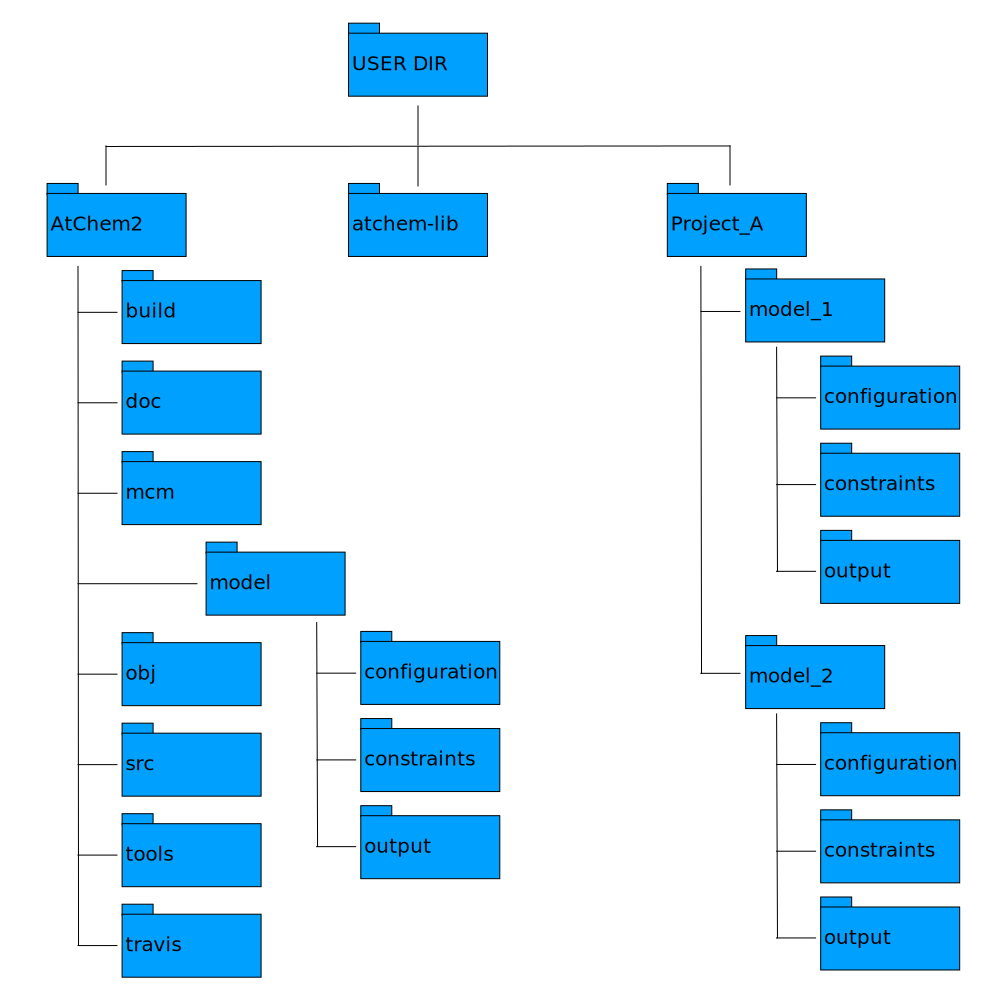
\includegraphics[width=0.85\textwidth]{model-setup.png}
  \caption{Example of a modelling setup, with an AtChem2 installation
    and a project directory containing two box-models.}
  \label{fig:setup}
\end{figure}

Fig.~\ref{fig:setup} shows a possible setup: a user directory (e.g.,
\texttt{\$HOME}) contains an AtChem2 installation -- with the default
\texttt{model/} directory -- plus a project directory
(\texttt{Project\_A}), which corresponds, for example, to a field
campaign or to a set of related experiments. The project directory
contains two different \texttt{model/} directories (\texttt{model\_1/}
and \texttt{model\_2/}), each with their own chemical mechanism,
configuration, constraints and output. In this case, the user can
build each model with the following commands~\footnote{The third
  argument is not specified in this example, so the default value
  (\texttt{\textasciitilde/AtChem2/mcm/}) will be used.}:

\begin{verbatim}
./build/build_atchem2.sh ~/Project_A/model_1/mechanism.fac
                         ~/Project_A/model_1/configuration/
\end{verbatim}

\begin{verbatim}
./build/build_atchem2.sh ~/Project_A/model_2/mechanism.fac
                         ~/Project_A/model_2/configuration/
\end{verbatim}

There are many different ways in which the \texttt{model/} directory
can be customized: for example, it is possible to keep all the
constraint files related to a project in one directory, thus avoiding
the need to have identical \texttt{constraints/} directories in each
\texttt{model/} directory. Each user has specific needs and personal
preferences; as long as the correct paths are passed to the
\texttt{build\_atchem2.sh} script (and to the executable, see
Sect.~\ref{sec:execute}), the model will compile and run.

Compilation is required only once for a given \texttt{.fac} file. If
the user changes the configuration files, there is no need to
recompile the model. Likewise, if the constraints files are changed,
there is no need to recompile the model. This is because the model
configuration and the model constraints are read by the executable at
runtime. However, if the user changes the \texttt{.fac} file, then the
shared library (\texttt{mechanism.so}) needs to be recompiled by
running the \texttt{build\_atchem2.sh} script again. The user may also
want, or need, to change the Fortran code (\texttt{src/*.f90}), in
which case the model needs to be recompiled. If the \texttt{.fac} file
has also been changed, the \texttt{build\_atchem2.sh} script must be
used; otherwise -- if only the Fortran code has been changed --
executing the command \verb|make| from the \maindir\ is enough to
recompile the model.

% -------------------------------------------------------------------- %
\section{Execute} \label{sec:execute}

The build process (Sect.~\ref{subsec:build-process} and
Sect.~\ref{sec:build}) creates an executable file called
\texttt{atchem2} in the \maindir. The executable file takes up to nine
arguments, corresponding to the \emph{relative paths} (with respect to
the \maindir) of the model configuration, the shared library, the
constraint files, and the model output:

\begin{enumerate}
\item the path to the model directory -- default:\\
  \texttt{model/}
\item the path to the directory for the model output -- default:\\
  \texttt{model/output}
\item the path to the directory with the configuration files -- default:\\
  \texttt{model/configuration/}.
\item the path to the directory with the model constraints -- default:\\
  \texttt{model/constraints/}
\item the path to the directory with the data files of constrained
  environment variables -- default:\\
  \texttt{model/constraints/environment/}
\item the path to the directory with the data files of constrained
  photolysis rates -- default:\\
  \texttt{model/constraints/photolysis/}
\item the path to the directory with the data files of constrained
  chemical species -- default:\\
  \texttt{model/constraints/species/}
\item the path to the directory with the MCM data files -- default:\\
  \texttt{mcm/}.
\item the path to the shared library -- default:\\
  \texttt{model/configuration/mechanism.so}.
\end{enumerate}

AtChem2 uses a series of input flags to pass the arguments to the
executable: \texttt{--model}, \texttt{--output},
\texttt{--configuration}, \texttt{--constraints},
\texttt{--env\_constraints}, \texttt{--photo\_constraints},
\texttt{--spec\_constraints}, \texttt{--mcm},
\texttt{--shared\_lib}. In addition, the input flag \texttt{--help}
displays an help message which shows the usage of the command line
arguments and of the input flags.

AtChem2 can be run simply by executing the command \verb|./atchem2|
from the \maindir, in which case the executable will assume that all
arguments have the default values. The equivalent command using the
input flags is:

\begin{verbatim}
./atchem2 --model=model/
          --output=model/output/
          --configuration=model/configuration/
          --constraints=model/constraints/
          --spec_constraints=model/constraints/species/
          --env_constraints=model/constraints/environment/
          --photo_constraints=model/constraints/photolysis/
          --shared_lib=model/configuration/mechanism.so
          --mcm=mcm/
\end{verbatim}

Not all flags have to be used, and the order in which they are used
does not matter. If a flag is not used, the executable assumes the
default value following a hierarchical directory structure. For
example, the following command assumes that a directory called
\texttt{output/} is present inside the \texttt{model/} directory, and
that three directories called \texttt{species/}, \texttt{environment/}
and \texttt{photolysis/} are present inside the \texttt{model/constraints/}
directory:

\begin{verbatim}
./atchem2 --model=model/
          --configuration=model/configuration/
          --constraints=model/constraints/
          --shared_lib=model/configuration/mechanism.so
\end{verbatim}

This approach gives the the user a lot of flexibility in the
organization of the modelling work and makes it possible to run
several models using the same executable with different
configurations, constraint sand chemical mechanisms. For example, the
following commands run the same model with two different
configurations and save the corresponding outputs in separate
directories:

\begin{verbatim}
./atchem2 --configuration=model/configuration_1/ --output=model/output_1/
./atchem2 --configuration=model/configuration_2/ --output=model/output_1/
\end{verbatim}

It is also possible to use configurations or constraints from
different models: for example, based on the setup shown in
Fig.~\ref{fig:setup}, the following command runs a model constrained
to the chemical species and environment variables of \texttt{model\_1/},
but constrained to the photolysis rates of \texttt{model\_2/}:

\begin{verbatim}
./atchem2 --configuration=model/configuration/
          --output=model/output/
          --spec_constraints=~/Project_A/model_1/constraints/species/
          --env_constraints=~/Project_A/model_1/constraints/environment/
          --photo_constraints=~/Project_A/model_2/constraints/photolysis/
\end{verbatim}

AtChem2 can be installed and run on High Performance Computing (HPC)
systems. This is recommended, especially for models with long runtimes
and/or many constraints. Each HPC system has its own rules and setup,
so it is not possible to give specific advice. Users should check the
local documentation or ask the system administrator; some information
about running AtChem2 on HPC systems can be found on the
\href{https://github.com/AtChem/AtChem2/wiki/Running-on-HPC}{wiki}.

% -------------------------------------------------------------------- %
\section{Output} \label{sec:output}

The model output is saved by default in the \texttt{model/output/}
directory. The location can be modified by changing the arguments of
the \texttt{atchem2} executable, as explained in
Sect.~\ref{sec:execute} (see also Sect.~\ref{subsec:model-directory}).
The frequency of the model output is determined by the following model
parameters, which are set in the \texttt{model.parameters} file
(Sect.~\ref{sec:model-parameters}):

\begin{itemize}
\item \textbf{step size} for the chemical species, the environment
  variables, the photolysis rates, the diagnostic variables.
\item \textbf{rates output step size} for the rate of production and
  destruction analysis (ROPA/RODA) of selected species.
\item \textbf{reaction rates output step size} (previously called
  \textbf{instantaneous rates}) for the reaction rates of all chemical
  reactions.
\end{itemize}

All AtChem2 output files are space-delimited text files with a one
line header containing the names of the variables. The first column of
each file is the model time (\texttt{t}) in seconds since midnight of
the start date~\footnote{Note that the \textbf{start date} is
  different than the \textbf{model start time}. The model start time
  indicates when the model begins its run and is in seconds since the
  midnight of the start date (Sect.~\ref{sec:model-parameters}).}:

\begin{itemize}
\item Environment variables and \cf{RO2} sum:\\
  \texttt{environmentVariables.output}
\item Concentrations of the chemical species:\\
  \texttt{speciesConcentrations.output}
\item Photolysis rates:\\
  \texttt{photolysisRates.output}
\item Latitude, longitude, solar angles and related parameters:\\
  \texttt{photolysisRatesParameters.output}
\item Loss and production rates of selected species:\\
  \texttt{lossRates.output}\\
  \texttt{productionRates.output}
\item Jacobian matrix (optional, see Sect.~\ref{sec:model-parameters}):\\
  \texttt{jacobian.output}
\item Error messages and diagnostic variables:\\
  \texttt{errors.output}\\
  \texttt{finalModelState.output}\\
  \texttt{mainSolverParameters.output}
\end{itemize}

In addition to the \texttt{.output} files, the reaction rates of every
reaction in the chemical mechanism are saved in the
\texttt{reactionRates/} directory -- called
\texttt{instantaneousRates/} in previous versions of AtChem
(Tab.~\ref{tab:atchem-dirs}) -- as one file for each model step, with
the name of the file corresponding to the output time in seconds.

The reaction rates files are useful for diagnostic purposes, but can
be cumbersome to process and analyze. In order to make it easier to
perform the rate of production and destruction analysis of chemical
species of particular interest -- i.e. those listed in
\texttt{outputRates.config} (Sect.~\ref{subsec:outputrates}) -- the
model produces the output files \texttt{productionRates.output} and
\texttt{lossRates.output}. These files contain the reaction rates of
production and destruction of the selected species in a human readable
format, illustrated in Fig.~\ref{fig:ropa}.

\begin{figure}[htb]
  \centering
  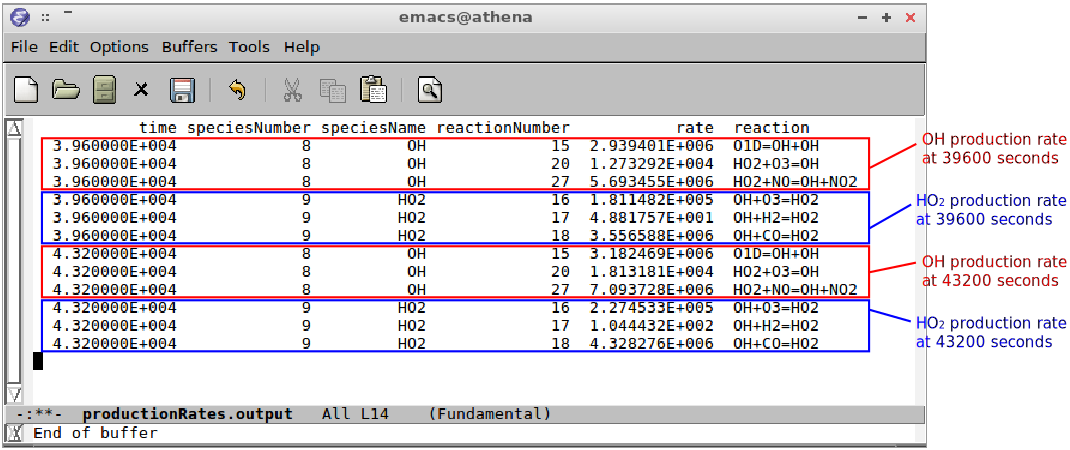
\includegraphics[width=0.95\textwidth]{output-rates.png}
  \caption{Format of the \texttt{productionRates.output} file. The
    \texttt{lossRates.output} file has a similar format.}
  \label{fig:ropa}
\end{figure}

While the model is running, diagnostic information is printed to the
terminal: this can be redirected to a log file using standard unix
commands. On HPC systems the submission script can usually take care
of redirecting the terminal printout to a log file (see the related
\href{https://github.com/AtChem/AtChem2/wiki/Running-on-HPC}{wiki page}).
A successful model run completes with a message similar to the one
shown in Sect.~\ref{sec:install}.
